\documentclass{article}
\usepackage[utf8]{inputenc}
\usepackage{natbib}
\usepackage{amsmath}

\title{Replicate : A Hybrid System Model of Seasonal Snowpack Water Balance}
\author{Fred Eisele }
\date{2014 December 12}

%% \usepackage[showframe=false]{geometry}
%% \geometry{verbose, tmargin=0pt, bmargin=90pt, lmargin=90pt, rmargin=90pt}
\usepackage{graphicx}
\usepackage{amsmath}
\usepackage{amsfonts}
\usepackage{xfrac}
\usepackage{subfigure}

\begin{document}

\maketitle

\section{Motivation for Work}

Systems with long time steps may be modeled with hybrid automata
\cite{kerkez2010swb}.
This project replicates part of the work involved with modeling
the seasonal snowpack water balance and the snow-water-equivalence (SWE).
The SWE is important in estimations of the water available
for consumption in the winter snowpack.
This is of particular importance in the desert west of the USA.
As policies are developed concerning water rights it
will be useful to have accurate models and simulations.

\section{Physical Model}

The problem space primarily concerns the Spring thaw.
We can assume that there is no additional snowfall,
no appreciable sublimation and that there is no
heat transfer by convection to the atmosphere.
Further we treat this as a bulk with instantaneous
heat conduction (assume no thermal resistance).
The conversion of the snowpack to run-off is due solely
to radiative effects, insolation, heating from the sun,
and night time cooling.

\subsection{Diurnal Insolation}

In the paper the insolation was obtained emperically.
For my purpose the solar intensity is modeled as a sine
function during the day and clipped for night.
Typical daily insolation values are about $3 \text{kW-hr/day}$.

\begin{align}
u(t)_{solar} &= a \sin{2 \pi t} \\
\int_0^{1 day} u(t)_{solar} dt &= \frac{a}{2 \pi} \\
  &\approx 3 \text{kW-hr/day} \\
a &\approx 30,000 kJ/day
\end{align}

This is coupled with a constant cooling to produce heating function.
\begin{align}
u(t)_{space} &\approx 0.1 \text{kW/$m^2$} \\
   &\approx 8600 \text{kJ/$m^2$-day} \\
u(t) &= 30,000 \sin{2 \pi t} - 8600 \text{kJ/$m^2$-day}
  \label{equ:power}
\end{align}


\subsection{Capacitive Heating}

The heat capacity of snow is the same as that of ice.

\begin{align}
\frac{dT}{dt} &= \frac{u(t)}{M_{snow} C_{snow}}
\label{eqn:heat-capacitance}
\end{align}
This is used only in the Frozen mode as that is
the only mode where the temperature changes.

\subsection{Melting}

The latent heat of fusion for snow is the same as for ice.
\begin{align}
\frac{dM_{water}}{dt} &= -\frac{dM_{ice}}{dt} \\
  &= \frac{u(t)}{L_f}
  \label{eqn:heat-latency}
\end{align}
This is not used in the Frozen mode as there is no water present.

\subsection{Compaction}

Snow is a mixture of ice and air.
The specific composition is varied and several models exist.
The compaction behavior over time is complex but can
be well described by formula.
Starting with the half-saturation formula where $A$ ($kg/m^2$) is the
maximum saturation level and $B$ ($days$) is the
half-saturation time.
Taking the derivative gives the compaction rate.

\begin{align}
\rho_{snow}(t) &= \frac{A}{1 + B/t} \\
\frac{d\rho_{snow}(t)}{dt} &= \frac{A B}{(B + t)^2} \\
\end{align}

Computing the time when a particular density is reached and
substituting gives a function for the compaction rate
as a function of density.

\begin{align}
t &= \frac{\rho_{snow} B}{A - \rho_{snow}} \\
\frac{d\rho_{snow}(t)}{dt}
    &= \frac{A}{B (1 + \frac{\rho_{snow}(t)}{A - \rho_{snow}(t)}) }
    \label{eqn:compaction}
\end{align}

Compaction occurs in all modes except in the
absence of a snowpack.


\subsection{Adsorbtion}

Snow acts as a sponge, adsorbing water into its matrix.
This fact distinguishes the thawing and melting modes.
The thawing mode is characterized by the snow's ability
to adsorb more water, while the melting mode is supersaturated
and additional conversion of ice into water results in run-off.
This idea is expressed in the volumetric water content of the snow,
$\theta_{snow}$.

\begin{align}
\theta_{snow} &= \frac{V_{water}}{V_{total}} \\
   &= \frac{M_{water}/ \rho_{water}}{M_{snow}/\rho_{snow}}
\end{align}

The maximum $\theta_{snow}$ signals the transition between
modes, designated $\theta_{r}$.
The mass of water in the saturated snowpack follows directly.
And, differentiating by parts once gives the rate that the water in the
snowpack is changing.

\begin{align}
M_{water}  &= \theta_{r} \rho_{water}
      \frac{M_{ice}}{\rho_{snow} - \theta_{r} \rho_{water}} \\
\frac{d M_{water}}{dt} &=  \theta_{r} \rho_{water}
   \left[ \frac{\frac{d M_{water}}{dt} (\rho_{snow} - \theta_{r} \rho_{water})
                  - M_{ice} \frac{d \rho_{snow}}{dt} }
          {(\rho_{snow} - \theta_{r} \rho_{water})^2} \right]
          \label{eqn:saturation}
\end{align}

Intuitively this relation makes sense.
A higher density in the snowpack results is a lower adsorbtivity.
These provide a sufficient physical model to construct the hybrid model.
The output of most interest in the report is the snow-water-equivalent (SWE).
This denotes the height of water that would result if the remaining
snow were converted to water.

\begin{equation}
swe(t) = \frac{M_{ice}(t) + M_{water}(t)}{\rho_{water}} \label{eqn:swe}
\end{equation}


\section{Hybrid Model}

The hybrid model is a bulk model for an arbitrary core
sample of the snowpack.

\begin{figure}[h!]
\centering
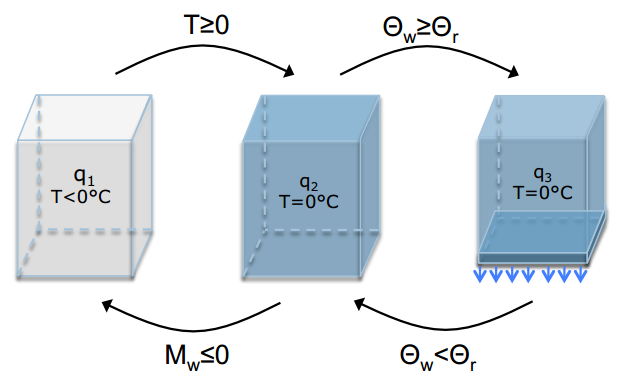
\includegraphics[scale=0.7]{discrete_modes.png}
\caption{The snowpack modes}
\label{fig:snowpack-modes}
\end{figure}

We start with the formal definition of the model.

\begin{align}
H &= (Q, X, Init, U, f, Dom, R, Y) \\
X &= \{x \in \mathbb{R}^4 \big| x = \left[ M_{ice}, M_{water}, \rho_{snow}, T \right]^T\}
\end{align}

\subsection{Discrete Model}

There are four discrete modes in this model.
It has two top level modes, one representing the absence
of snow, and the other representing the presence of a snowpack.
The snowpack mode is further discriminated into three modes:
frozen, thawing and melting.
Frozen indicates the absence of water in the snow matrix,
only ice and air are present.
Thawing indicates that the ice and water are in a phase change condition;
all the water present is adsorbed by the snow matrix.
Melting indicates a supersaturated state where the
volumetric water content of the snowpack is at a maximum.

\begin{align}
Q &= \{q_0, q_1, q_2, q_3\} \\
  &= \{\text{empty}, \text{frozen}, \text{thawing}, \text{melting}\}
\end{align}

\begin{align}
Dom_{empty} &= \{x \in X \big| M_{ice} <= 0\} \\
Dom_{frozen} &= \{x \in X \big| T <= 0\} \\
Dom_{thawing} &= \{x \in X \big| T >= 0
    \wedge 0 < M_{water} <
    \theta_{r} \rho_{water} \frac{M_{ice} + M_{water}}{\rho_{snow}}\} \\
Dom_{melting} &= \{x \in X \big|  M_{water} >=
    \theta_{r} \rho_{water} \frac{M_{ice} + M_{water}}{\rho_{snow}}\}
\end{align}

The initial states are arbitrarily chosen but must meet
the following criteria regardless of the initial mode.

\begin{align}
M_{ice} &>= 0 \\
M_{water} &>= 0 \\
M_{water} &<= \theta_{r} \rho_{water} \frac{M_{ice} + M_{water}}{\rho_{snow}} \\
\rho_{snow} &>= 0 \\
\rho_{snow} &<= A \text{ ( the maximum saturation level) } \\
T &<= 0
\end{align}

The domain also suggests the reset relations.
\begin{align}
R(empty,x) &= (frozen, x)  & \textrm{  if $0 < M_{ice}$ } \\
R(frozen,x) &= (thawing,x) & \textrm{  if $0 \le T$ } \\
R(thawing,x) &= (frozen,x) & \textrm{  if $T \le 0$ } \\
R(thawing,x) &= (melting,x) & \textrm{  if
   $\theta_{r} \le \frac{M_{water} / \rho_{water} }
        {(M_{ice} + M_{water}) / \rho_{snow}}$  } \\
R(melting,x) &= (thawing,x) & \textrm{  if
      $\frac{M_{water} / \rho_{water} }
        {(M_{ice} + M_{water}) / \rho_{snow}} < \theta_{r}$  } \\
R(q,x) &= (empty, x) & \textrm{otherwise}
\end{align}

Notice the implementation issue with the $R(frozen,x) \to (thawing,x)$ and
$R(thawing,x) \to (frozen,x)$ the implementation will need to
force at least one time step before leaving.


\subsection{Dynamic Model}

When there is no snowpack some of the values in $x$ are undefined
and are arbitrarily set to zero.
The mass of ice remaining is clearly $M_{ice} = 0$.

In each case the power is given by Equation \ref{eqn:power}.

\begin{equation}
f_{empty}(t,x(t),u(t)) =
  \begin{bmatrix} 0 \\ 0 \\ 0 \\ 0 \end{bmatrix}
\end{equation}

In each of the remaining cases the snowpack density, $p_{snow}$
increases due to compaction, Equation: \ref{eqn:compaction}.

When in the sub-zero, frozen, mode  there is no change in mass composition.
The snow does compact and the temperature is free to change.

\begin{equation}
f_{frozen}(t,x(t),u(t)) =
  \begin{bmatrix}
     0 \\ 0 \\
     Equation: \ref{eqn:compaction} \\
     Equation: \ref{eqn:heat-capacitance}
  \end{bmatrix}
\end{equation}

In the thawing mode the temperature is locked to the material
phase transition temperature ($0 \degree C$).

\begin{equation}
f_{thawing}(t,x(t),u(t)) =
  \begin{bmatrix}
     - Equation: \ref{eqn:heat-latency} \\
     Equation: \ref{eqn:heat-latency} \\
     Equation: \ref{eqn:compaction} \\
     0
  \end{bmatrix}
\end{equation}

\begin{equation}
f_{melting}(t,x(t),u(t)) =
  \begin{bmatrix}
     - Equation: \ref{eqn:heat-latency} \\
     Equation: \ref{eqn:saturation} \\
     Equation: \ref{eqn:compaction} \\
     0
  \end{bmatrix}
\end{equation}

The output of the system, $Y$ is given by Equation \ref{eqn:swe}.


\section{Work Performed}

Using the hybrid model and based on the recommended
Stateflow\textregistered Simulink\textregistered
design pattern \citep{matlab2009ssdp} I constructed a
hybrid model.

Several variations on inputs were examined, two of which follow.
In each of these cases the mass is in kg, the time in in days,
the density is in kg/$m^3$, energy (insolation) is in
kJ/$m^2$/day, and height (SWE) is in meters.

\begin{figure}
\centering
\mbox{
\subfigure{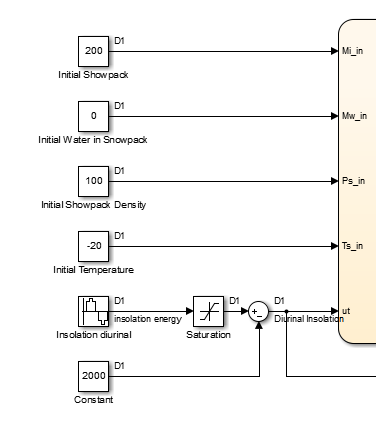
\includegraphics[width=2in]{melting_trend_input.png}} \quad
\subfigure{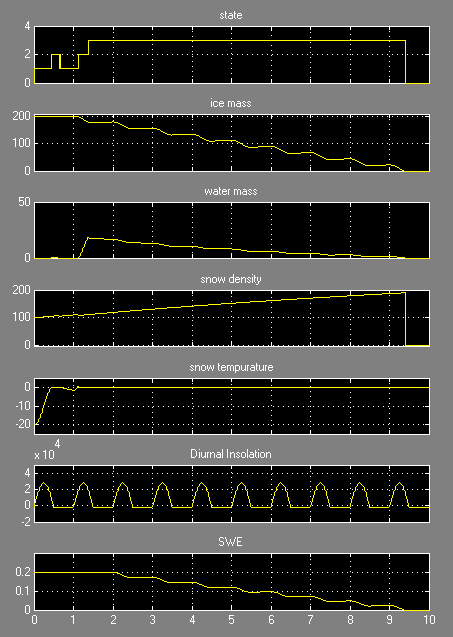
\includegraphics[width=4in]{melting_trend_output.png}}
}
\caption{Snowpack consistently melting} \label{fig:consistent-melting}
\end{figure}

In this example, Figure \ref{fig:consistent-melting}, the energy is diurnal.
Notice that the temperature increases more rapidly than the melt.
This is due to the fact that the latent heat of fusion is much
greater than the heat capacity for water.
Note that the heat lost at night is not sufficiently large
to move the mode back into thawing or freezing.
With this in mind, a simulation was performed with a much
higher nightly radiation.


\begin{figure}
\centering
\mbox{
\subfigure{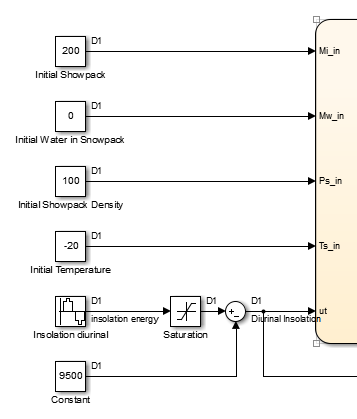
\includegraphics[width=2in]{refreeze_trend_input.png}} \quad
\subfigure{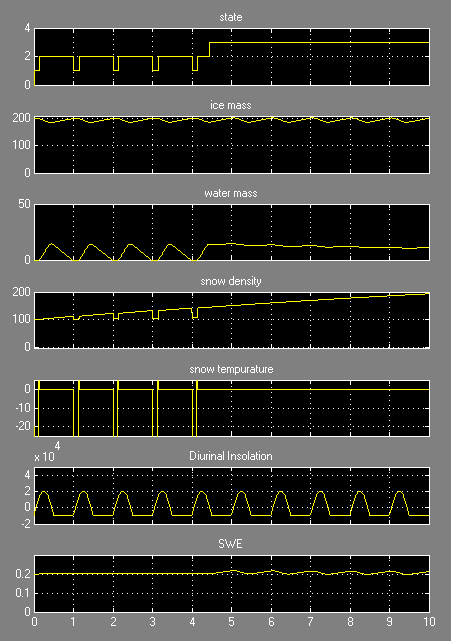
\includegraphics[width=4in]{refreeze_trend_output.png}}
}
\caption{Snowpack thawing and refreezing at night} \label{fig:refreezing-melt}
\end{figure}

In Figure \ref{fig:refreezing-melt} the general behavior looks as expected
with the water in the snowpack refreezing each night until
the system enters the melting mode.


\section{Modeling Issues}

There are several ways to model systems such as this,
each with their adavantages and drawbacks.
The model using Simulink\textregistered models supervised
by a Stateflow\textregistered model and driven by a
Simulink\textregistered model was choosen as it
closely imitates the formal hybrid model.
It has the drawback of requiring the transfer of
state information between integrators which makes use
of the reset with its added complexity.

The other significant issue is the proper calibration of the model.
Typically the models produced with
Stateflow\textregistered Simulink\textregistered are working
with time frames in the one second region.
This problem uses time frames in the hour or day region.

A minor issue is that the paper does not describe
the input in much detail.
The data they use is that recorded in various surveys.
This will be approximated in my model with a sine wave
that immitates the diurnal insolation with the trough
giving up energy.

There were a few minor errors in the equations in
paper that were corrected.


\section{Physical Constants and Conditions}

\begin{align}
u(t) &= a \sin{2 \pi t} - c_{rad} \\
 &= - c_{rad} \\
U(t) &= \frac{a \cos{2 \pi t}}{2 \pi} |_0^{1/2} - c_{rad} t |_0^1 \\
  &= 3 \text{ kW-hr/$m^2$ } \\
  &= 10,800 \text{ kJ/$m^2$ } \\
c_{rad} &= 800 \text{ kJ/$m^2$-day } \\
a &= (10,800 - c_{rad}) \times 2 \pi \text{ kJ/$m^2$-day } \\
 &= 20,000 \pi \text{ kJ/$m^2$-day } \\
 &\approx 63,000 \text{ kJ/$m^2$-day }
\end{align}

Where $t$ is measured in days.
$A$ is the average daily insolation.
A reasonable, Springtime, value for $A$ is near $3 \text{kW-hr}/m^2$.

\begin{align}
 C_{ice} &= 2.05 \text{ kJ/kg-K} \\
 C_s &= C_{ice} \\
\theta_r &= 0.01 \\
L_f &= 334 \text{ kJ/kg} \\
\rho_w &= 1000 \text{ kg/$m^3$} \\
A &= 450 \text{ kg/$m^3$} \\
B &= 20 \text{ days}
\end{align}


 \section{Conclusion}

 This problem shows that natural systems may be effectively
 modelled using hybrid-automata.
 Some areas that could be extended would include models
 for simultaneous snow accumulation.


\bibliographystyle{plain}
\bibliography{references}

\end{document}
